\documentclass{standalone}
\usepackage{tikz}
\usepackage{ctex,siunitx}
\setCJKmainfont{Noto Serif CJK SC}
\usepackage{tkz-euclide}
\usepackage{amsmath}
\usetikzlibrary{patterns, calc,3d}
\usetikzlibrary {decorations.pathmorphing,decorations.pathreplacing,decorations.shapes}
\tikzset{label style/.append style={font=\small}}
\begin{document}
\small
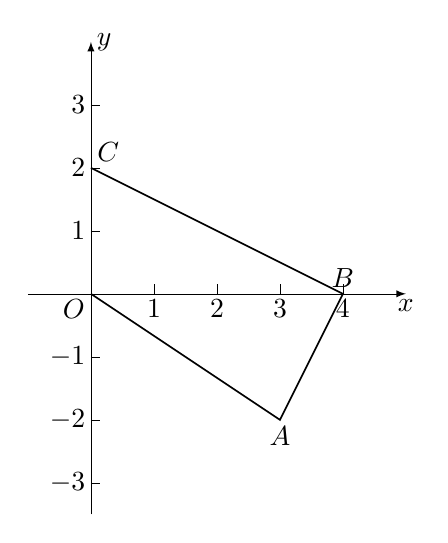
\begin{tikzpicture}[>=latex,scale=0.8,inner sep=2pt]
  \draw[very thin,->](-1,0)--(5,0)node[below]{$x$};
  \draw[very thin,->](0,-3.5)--(0,4)node[right]{$y$};
  \node at (0,0)[below left]{$O$};
  \foreach \x in {1,2,3,4}
  {\draw[very thin](\x,0)node[below]{$\x$}--++(0,0.15);}
  \foreach \x in {1,2,3}
  {
    \draw[very thin](0,\x)node[left]{$\x$}--++(0.15,0);
    \draw[very thin](0,-\x)node[left]{$-\x$}--++(0.15,0);
  }
  \draw[semithick](0,0)--(3,-2)node[below]{$A$}--(4,0)node[above]{$B$}--(0,2)node[above right]{$C$};
\end{tikzpicture}
\end{document}